\subsection{Learned transformations generalize to new sections and granularities}
\label{sec:granularity-transfer}
\label{sec:scale-continuum}

The preceding results concern directly encoded representations. We now ask whether the learned relationships themselves support prediction, first at trained target granularities on new sections and then at intermediate granularities absent from training. In both tests, a prediction uses only the source molecular state and the requested granularity. Direct encodings of the actual target neighborhoods provide the scoring references.

\paragraph{Trained relationships transfer to held-out sections.}
Across all eight held-out sections, transformed states have lower target MSE than unchanged fine states for each trained granularity pair (Figure~\ref{fig:generalization-summary}A). Equal-section mean reductions are 21.3\%, 27.0\%, and 11.8\% for $8\to32$, $8\to128$, and $32\to128$, respectively. Correct fine--predicted-coarse pairings also have lower joint-distribution discrepancy than shuffled pairings in every section and direction, including evaluation with projections unused in training (Figure~\ref{fig:generalization-summary}B). Shuffling preserves the predicted coarse marginal distribution but disrupts its association with the fine source. Together, the error reduction and pairing control support transferable, location-dependent fine--coarse relationships (Appendix~\ref{app:granularity-transfer}).

\paragraph{Discrete supervision supports unseen-granularity queries.}
With both encoder and transition frozen after training only at 8, 32, and 128, we query six unseen granularities---12, 16, 24, 48, 64, and 96---from the same $e_{i,8}$. Predictions reduce target MSE in all 48 held-out section--granularity conditions (Figure~\ref{fig:generalization-summary}A). Averaging prediction and unchanged-source errors over the six targets within each section, then averaging the section-level relative reductions, gives a 21.96\% reduction. Intermediate encodings are used only for evaluation. The same learned transformation can therefore predict descriptions at observation ranges beyond the discrete training set; all section-level errors and the separate PCA illustrations are provided in Appendix~\ref{app:unseen-state-detail}.

\begin{figure}[!htbp]
\centering
\begin{minipage}[t]{0.625\linewidth}
\centering\vspace{0pt}
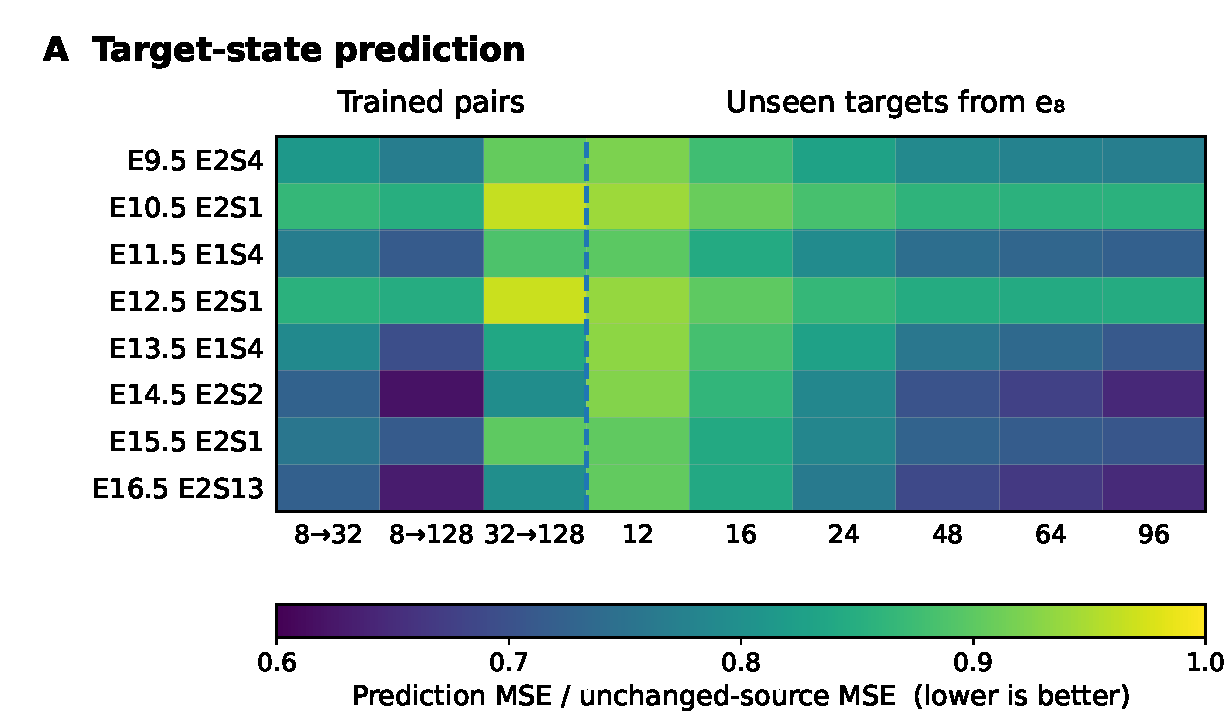
\includegraphics[width=\linewidth]{figures/results_generalization_matrix.pdf}
\end{minipage}\hfill
\begin{minipage}[t]{0.355\linewidth}
\centering\vspace{0pt}
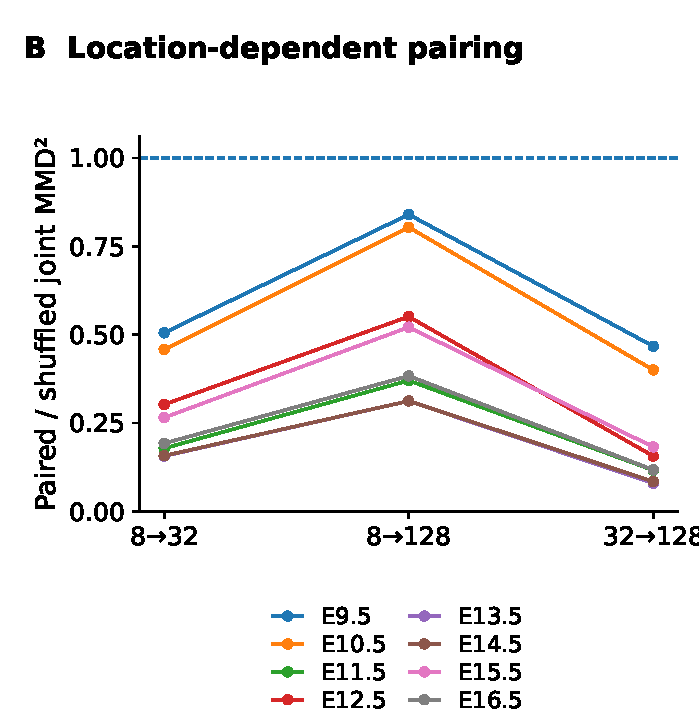
\includegraphics[width=\linewidth]{figures/results_pairing_control.pdf}
\end{minipage}
\caption{\textbf{Transformation generalization across held-out sections and observation granularities.} \textbf{A}, Target-MSE ratios for the three trained source--target pairs (left) and six unseen targets queried from $e_8$ (right). Each cell compares prediction with an unchanged source against the same directly encoded target. Trained-pair evaluation uses all section positions; unseen-target evaluation uses 1,024 fixed positions per section. All 24 trained-pair and 48 unseen-target ratios are below one. \textbf{B}, Correct-pair to shuffled-pair joint-MMD ratios for the trained pairs, averaged over four batches and eight projections unused in training. Each line is one held-out section. Values are from Tables~\ref{tab:granularity-transfer-sections} and~\ref{tab:ode-intermediate-sections}.}
\label{fig:generalization-summary}
\end{figure}

\paragraph{Continuous parameterization improves a matched prediction task.}
In a separate comparison on a shared frozen encoder, the neural ODE reduces mean unseen-granularity MSE by 10.86\% relative to a granularity-conditioned residual MLP, with lower error on all eight held-out sections. Both heads use the same source states and encoded targets (Appendix~\ref{app:transition-comparison}). This matched comparison supports the continuous parameterization; the preceding held-out tests establish the predictive capability of the jointly trained model.
\FloatBarrier
